\documentclass{article}

% Idioma
\usepackage[spanish]{babel}

% márgenes y formato
\usepackage[a4paper,top=2cm,bottom=2cm,left=3cm,right=3cm,marginparwidth=1.75cm]{geometry}
\usepackage{parskip}

% Otros paquetes importantes
\usepackage{amsmath}
\usepackage{amssymb}
\usepackage{graphicx}
\usepackage[colorlinks=true, linkcolor=black, urlcolor=blue]{hyperref}

% PARA APUNTES: darkmode
% \usepackage{darkmode}
% \enabledarkmode

% Titulo y autor
\title{Métodos de Taylor para EDOs}
\author{Álvaro Hernández Riquelme}
\date{\today}

\begin{document}

%%%%%%%%%%%%%%%%%%%%%%%%%%%%%%%%%%

\maketitle
\tableofcontents
\newpage

\section{Introducción}

Nuestra ecuación diferencial será:

\begin{equation}
y'(x) = 4x + y(x)^2
\end{equation}

con la condición inicial de:

\begin{equation}
y(0) = 1
\end{equation}

y el punto final:

\begin{equation}
b = 0.04
\end{equation}
Se resolverán los ejercicios propuestos.

\section{Primeros ejercicios}

\subsection{Aplicar un paso de longitud con Taylor de orden 1}

Para este primer apartado, se nos pide aplicar un paso con el método de Taylor de orden 1.
Con $h=0.04$ y orden 1, calculamos la primera derivada de $y(x)$ en el punto inicial. La función, como hemos visto antes, es $y'(x) = 4x + y(x)^2$.

Sustituyendo por el valor de la condición inicial $x=0, y(0)=1$:

\begin{equation}
y'(0) = 4 \cdot 0 + (1)^2 = 1
\end{equation}
Aplicando la formula (19) dada en teoria para $n=1$, que corresponde al método de Euler explícito, obtenemos la expresión:
\begin{equation}
y_1 = y(0) + h \cdot y'(0)
\end{equation}
Sustituyendo los valores calculados:
\begin{align*}
y_1 &= 1 + 0.04 \cdot 1 \\
&= 1 + 0.04 \\
&= \boxed{1.04}
\end{align*}

\subsection{Aplicar un paso de longitud con Taylor de orden 2}

Ahora, con $h=0.04$ y orden 2, necesitamos la segunda derivada de $y(x)$, que se obtiene derivando la EDO:
\begin{equation}
y''(x) = \frac{d}{dx}(4x + y(x)^2) = 4 + 2 \cdot y(x) \cdot y'(x)
\end{equation}
Sustituyendo por los valores en el punto inicial, $y(0)=1$ y $y'(0)=1$:
\begin{equation}
y''(0) = 4 + 2 \cdot y(0) \cdot y'(0) = 4 + 2 \cdot 1 \cdot 1 = 6
\end{equation}
Aplicando la formula (19) de la teoría para $n=2$:
\begin{equation}
y_1 = y(0) + h \cdot y'(0) + \frac{h^2}{2} \cdot y''(0)
\end{equation}
Sustituyendo los valores:
\begin{align*}
y_1 &= 1 + 0.04 \cdot 1 + \frac{0.04^2}{2} \cdot 6 \\
&= 1.04 + \frac{0.0016}{2} \cdot 6 \\
&= 1.04 + 0.0048 \\
&= \boxed{1.0448}
\end{align*}

\subsection{Aplicar un paso de longitud con Taylor de orden 3}

Con $h=0.04$ y orden 3, calculamos la tercera derivada de $y(x)$:
\begin{equation}
y'''(x) = \frac{d}{dx}(4 + 2y'y) = 2(y')^2 + 2yy''
\end{equation}
Sustituyendo con los valores ya conocidos en el punto inicial ($y(0)=1, y'(0)=1, y''(0)=6$):
\begin{equation}
y'''(0) = 2(y'(0))^2 + 2 \cdot y(0) \cdot y''(0) = 2 \cdot 1^2 + 2 \cdot 1 \cdot 6 = 2 + 12 = 14
\end{equation}
Aplicando la formula (19) para $n=3$:
\begin{equation}
y_1 = y(0) + h \cdot y'(0) + \frac{h^2}{2} \cdot y''(0) + \frac{h^3}{6} \cdot y'''(0)
\end{equation}
Sustituyendo los valores:
\begin{align*}
y_1 &= 1 + 0.04 \cdot 1 + \frac{0.04^2}{2} \cdot 6 + \frac{0.04^3}{6} \cdot 14 \\
&= 1.0448 + \frac{0.000064}{6} \cdot 14 \\
&= 1.0448 + 0.000149333... \\
&= \boxed{1.044949333}
\end{align*}

%\subsection{Ejercicio 4}
%Para un paso con $h=0.04$ y orden 4, calculamos la cuarta derivada de $y(x)$:
%\begin{equation}
%y''''(x) = \frac{d}{dx}(2(y')^2 + 2yy'') = 4y'y'' + 2y'y'' + 2yy''' = 6y'y'' + %2yy'''
%\end{equation}
%Sustituyendo con los valores en el punto inicial ($y(0)=1, y'(0)=1, y''(0)=6, y'''%(0)=14$):
%\begin{equation}
%y''''(0) = 6 \cdot y'(0) \cdot y''(0) + 2 \cdot y(0) \cdot y'''(0) = 6 \cdot 1 %\cdot 6 + 2 \cdot 1 \cdot 14 = 36 + 28 = 64
%\end{equation}
%Aplicando la formula (19) para $n=4$:
%\begin{equation}
%y_1 = y(0) + h y'(0) + \frac{h^2}{2} y''(0) + \frac{h^3}{6} y'''(0) + \frac{h^4}%{24} y''''(0)
%\end{equation}
%Sustituyendo los valores:
%\begin{align*}
%y_1 &= 1.044949333 + \frac{0.04^4}{24} \cdot 64 \\
%&= 1.044949333 + \frac{0.00000256}{24} \cdot 64 \\
%&= 1.044949333 + 0.000006826... \\
%&= \boxed{1.0450176}
%\end{align*}

\subsection{¿Cual es el único caso que no derivamos la ecuación diferencial?}

El unico caso en el que no derivamos la ecuación diferencial es en el caso del orden 1, ya que ahí usamos la condición inicial únicamente, y no hay necesidad de obtener ninguna otra derivada.

\subsection{¿Fueron útiles los valores de Taylor de grados menores?}

Todas las derivadas han sido usadas a la hora de obtener la ecuación en un orden superior. Se puede apreciar que para calcular $y^{(j)}(x)$ es necesario conocer las derivadas de orden inferior $y^{(k)}(x)$, es decir, para $y^{(3)}(x)$ se necesitan $y^{(2)}(x)$ y $y^{(1)}(x)$. (NOTA: normalmente no usamos números para el orden de la derivada pero de esta forma se entiende mejor)

\section{Segundos ejercicios}

\subsection{Dos pasos en Euler explícito}

A partir de este ejercicio se usará $N=2$ pasos en el intervalo $[0, 0.04]$, por lo que la longitud de cada paso es $h=\frac{0.04}{2}=0.02$. Se aplica el método de Taylor de orden 1.

Usamos los cálculos iniciales con $x_0=0, y_0=1$ y el nuevo $h=0.02$.
\begin{equation}
y'(0) = 1
\end{equation}
\begin{equation}
y_1 = y(0) + h \cdot y'(0) = 1 + 0.02 \cdot 1 = 1.02
\end{equation}

Nuestro nuevo punto inicial será $(x_1, y_1) = (0.02, 1.02)$. El cálculo de la solución será:


\begin{equation}
y(0.02) = 1.02
\end{equation}
Así que la derivada en ese punto será:
\begin{equation}
y'(0.02) = 4 \cdot 0.02 + y(0.02)^2 = 0.08 + 1.02^2 = 0.08 + 1.0404 = 1.1204
\end{equation}
Finalmente, la aproximación en $x=0.04$ es:
\begin{align*}
y_2 &= y(0.02) + h \cdot y'(0.02) \\
&= 1.02 + 0.02 \cdot 1.1204 \\
&= 1.02 + 0.022408 \\
&= \boxed{1.042408}
\end{align*}

\subsection{Dos pasos con Taylor de orden 2}
Se aplica el método de Taylor de orden 2 con $h=0.02$.

Recordando lo obtenido para el punto inicial: $y'(0)=1$ y $y''(0)=6$.

\begin{equation}
y_1 = y(0) + h \cdot y'(0) + \frac{h^2}{2} \cdot y''(0)
\end{equation}
\begin{align*}
y_1 &= 1 + 0.02 \cdot 1 + \frac{0.02^2}{2} \cdot 6 \\
&= 1.02 + \frac{0.0004}{2} \cdot 6 \\
&= 1.02 + 0.0012 = 1.0212
\end{align*}

El nuevo punto de partida es $(x_1, y_1) = (0.02, 1.0212)$.
Calculamos las derivadas en este nuevo punto:
\begin{gather}
y'(0.02) = 4(0.02) + (1.0212)^2 = 0.08 + 1.04284944 = 1.12284944 \\
y''(0.02) = 4 + 2 \cdot y(0.02) \cdot y'(0.02) = 4 + 2 \cdot 1.0212 \cdot 1.12284944 = 6.29178
\end{gather}
Finalmente, calculamos $y_2$:
\begin{align*}
y_2 &= y(0.02) + h \cdot y'(0.02) + \frac{h^2}{2} \cdot y''(0.02) \\
&= 1.0212 + 0.02 \cdot 1.12284944 + \frac{0.02^2}{2} \cdot 6.29178 \\
&= \boxed{1.04491565}
\end{align*}

\subsection{Dos pasos con Taylor de orden 3}
Se aplica el método de Taylor de orden 3 con $h=0.02$.

Derivadas en el punto inicial: $y'(0)=1, y''(0)=6, y'''(0)=14$.
\begin{equation}
y_1 = y(0) + h y'(0) + \frac{h^2}{2} y''(0) + \frac{h^3}{6} y'''(0)
\end{equation}
\begin{align*}
y_1 &= 1 + 0.02 \cdot 1 + \frac{0.02^2}{2} \cdot 6 + \frac{0.02^3}{6} \cdot 14 \\
&= 1.0212 + \frac{0.000008}{6} \cdot 14 \\
&= 1.0212 + 0.000018667 = 1.021218667
\end{align*}

Nuevo punto inicial $(x_1, y_1) = (0.02, 1.021218667)$.
Calculamos las derivadas necesarias en este punto:
\begin{gather}
y'(0.02) = 4(0.02) + (1.021218667)^2 = 1.1228875 \\
y''(0.02) = 4 + 2(1.021218667)(1.1228875) = 6.29196 \\
y'''(0.02) = 2(1.1228875)^2 + 2(1.021218667)(6.29196) = 15.3708
\end{gather}
Finalmente, calculamos $y_2$:
\begin{align*}
y_2 &= y(0.02) + h y'(0.02) + \frac{h^2}{2} y''(0.02) + \frac{h^3}{6} y'''(0.02) \\
&= 1.021218667 + 0.02(1.1228875) + \frac{0.0004}{2}(6.29196) + \frac{0.000008}{6}(15.3708) \\
&= \boxed{1.0449553}
\end{align*}


\subsection{Para el primero de los dos pasos, ¿fueron útiles los valores de los polinomios de Taylor de grados más bajos? }


Sí. Para el primer paso de los ejercicios 6, 7 y 8, se parte siempre de la misma condición inicial ($x_0=0, y_0=1$). Esto tiene dos implicaciones:

Las derivadas de la función en el punto inicial ($y'(0), y''(0), y'''(0)$, etc.) son las mismas que se calcularon para los ejercicios 1, 2 y 3. No tuve que volver a calcularlas.

La propia fórmula de Taylor se va acumulando. El polinomio de orden $n$ se construye añadiendo un término al polinomio de orden $n-1$.

\subsection{¿Y para el segundo de los dos pasos?}

No, en este caso no fueron útiles. El segundo paso comienza en un nuevo punto $(x_1, y_1)$, donde el valor $y_1$ es una aproximación que depende del método usado en el primer paso. Por ejemplo, el punto de partida para el segundo paso del Ejercicio 7 es diferente al del Ejercicio 8.

Debido a que el punto inicial del segundo paso es distinto en cada caso, es necesario recalcular todas las derivadas ($y'(x_1), y''(x_1)$, etc.) atendiendo a los nuevos valores de $x_1$ e $y_1$. Por lo tanto, los valores calculados en el primer paso no se pueden reutilizar para el segundo.

\section{Ejercicios finales}

Para estos tres siguientes ejercicios, simplemente se mostrará la salida de MAXIMA al llamar a la función \verb|Taylor_EDO| con los parámetros que se piden, ya que anteriormente ya hemos visto cómo se calcularía de forma manual.

Ahora llamamos con $N=4$ usando las funciones propuestas de MAXIMA:

\subsection{4 Pasos y h=0.01 con Euler explícito}

\begin{figure}[h]
    \centering
    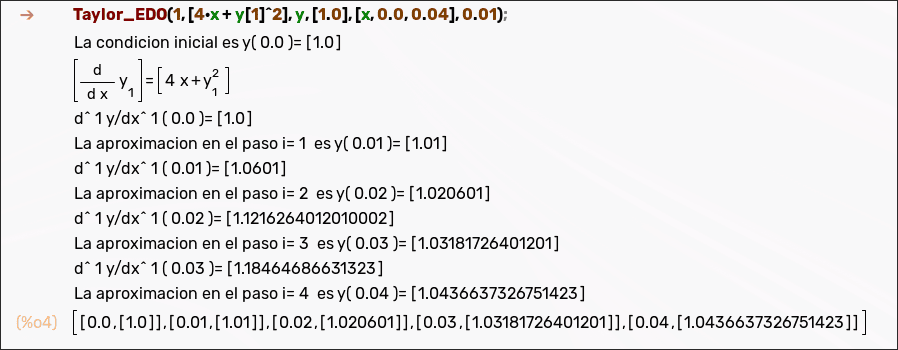
\includegraphics[width=0.8\textwidth]{src/taylor1.png}
    \caption{Primera salida de MAXIMA}
    \label{fig:maxima_output}
\end{figure}

\subsection{4 Pasos y h=0.01 con Taylor de orden 2}

\begin{figure}[h]
    \centering
    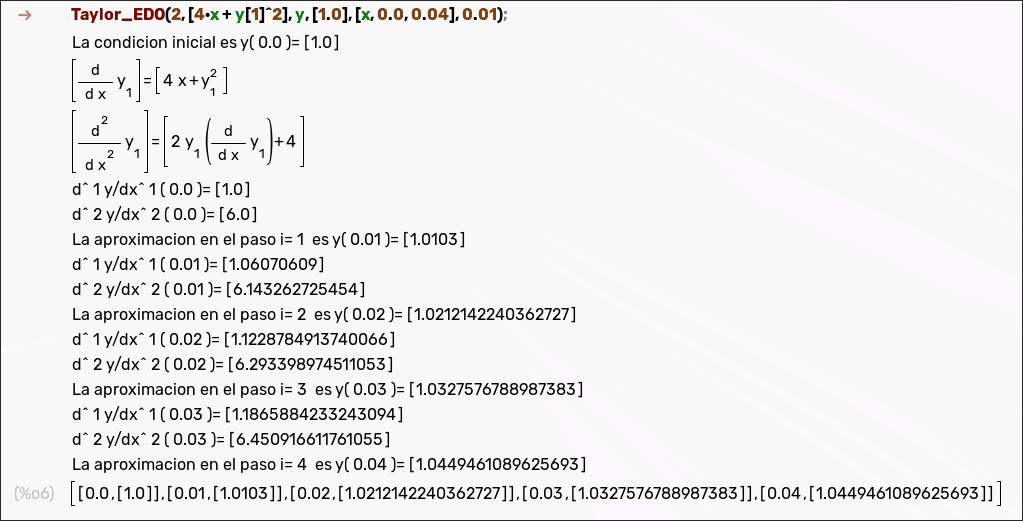
\includegraphics[width=0.8\textwidth]{src/taylor2.png}
    \caption{Segunda salida de MAXIMA}
    \label{fig:maxima_output2}
\end{figure}


\newpage


\subsection{4 Pasos y h=0.01 con Taylor de orden 3}

\begin{figure}[h]
    \centering
    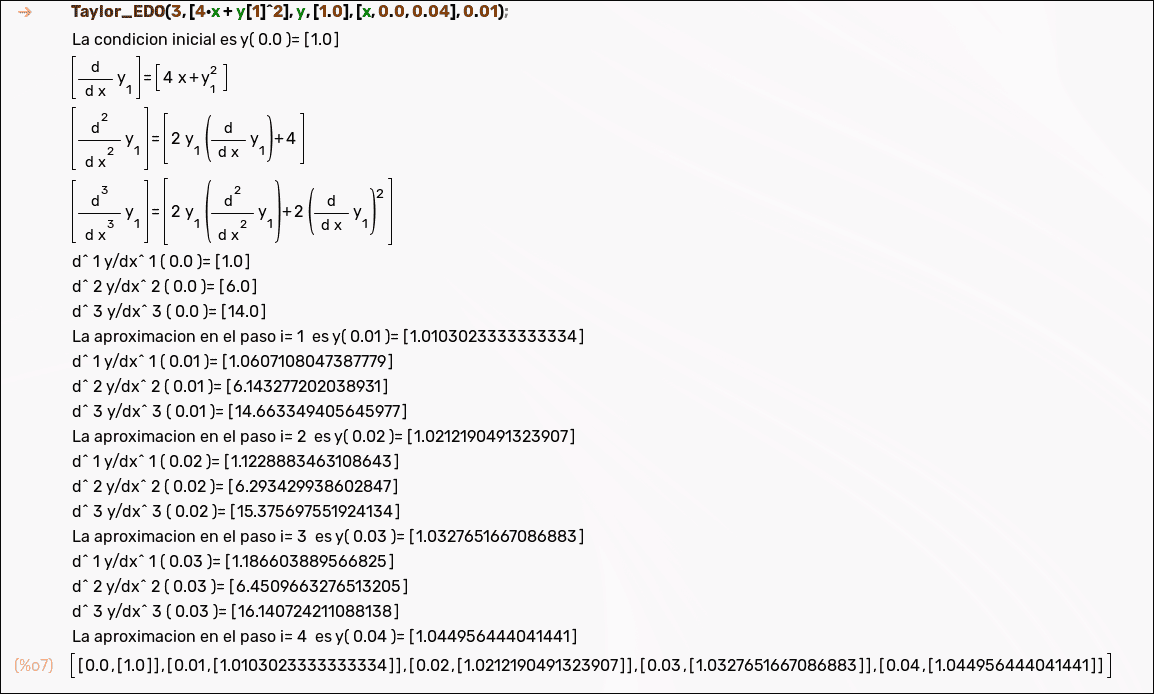
\includegraphics[width=0.8\textwidth]{src/taylor3.png}
    \caption{Última salida de MAXIMA}
    \label{fig:maxima_output3}
\end{figure}


\subsection{ ¿Consideras que las aproximaciones son parecidas o hay alguna dispar?}

Al comparar las 9 aproximaciones obtenidas para $y(0.04)$, se observa que la mayoría de los valores son bastante cercanos entre sí, especialmente los de orden 2 y 3. Aunque las diferencias se notan más en los cálculos realizados con el método de Taylor de orden 1 (método de Euler).

\subsection{De las 9 aproximaciones, ¿cuál necesitó más cálculos?}

De todas las aproximaciones, el ejercicio 13 (sección 4.3 en este documento) combina el orden más alto solicitado ($n=3$) con el mayor número de pasos ($N=4$), lo que lo convierte en el más laborioso. En cada uno de los 4 pasos hay que evaluar la función y sus tres primeras derivadas en un nuevo punto, a diferencia de otros métodos con menos pasos o de menor orden.

\subsection{De las 9 aproximaciones, ¿cuál crees que es la más precisa?}

La aproximación que se consideraría más precisa es también la del \textbf{Ejercicio 13} (orden 3, $h=0.01$).

La teoría de los métodos numéricos para EDOs indica que el error global de la aproximación disminuye al aumentar el orden del método y al reducir el tamaño del paso $h$. Al combinar el orden más alto ($n=3$) con el tamaño de paso más pequeño ($h=0.01$), se minimiza el error de truncamiento, resultando en la solución más cercana al valor real de $y(0.04)$.

\subsection{Resta la aproximación que hayas considerado más precisa a las otras}


Usando el valor del Ejercicio 13 como la mejor aproximación a la solución real, es decir, $y(0.04) \approx 1.044956$, calculamos el error estimado para las otras 8 aproximaciones:


\begin{itemize}
    \item \textbf{Error Ej. 1 ($h=0.04, n=1$):} $|1.044956 - 1.04| = 0.004956$
    \item \textbf{Error Ej. 2 ($h=0.04, n=2$):} $|1.044956 - 1.0448| = 0.000156$
    \item \textbf{Error Ej. 3 ($h=0.04, n=3$):} $|1.044956 - 1.044949333| \approx 0.00000667$
    \item \textbf{Error Ej. 6 ($h=0.02, n=1$):} $|1.044956 - 1.042408| = 0.002548$
    \item \textbf{Error Ej. 7 ($h=0.02, n=2$):} $|1.044956 - 1.04491535| \approx 0.00004065$
    \item \textbf{Error Ej. 8 ($h=0.02, n=3$):} $|1.044956 - 1.0449553| = 0.0000007$
    \item \textbf{Error Ej. 11 ($h=0.01, n=1$):} $|1.044956 - 1.043663| = 0.001293$
    \item \textbf{Error Ej. 12 ($h=0.01, n=2$):} $|1.044956 - 1.044946| = 0.00001$
\end{itemize}


\end{document}
